\chapter{观察世界：五种感官}\label{ch:g1:five-senses}

头顶某处，有一只鸟在歌唱。面包闻起来是热的。路面
隔着袜子摸上去是冷的。做任何其他事情之前，物理学
先要看、听、摸：本章讲的是用五种感官
观察世界 --- 以及它们会如何捉弄我们。

\section{五种感官}

\begin{definition}[五种感官]\label{def:g1:five-senses:senses}
\emph{感官}\index{感官}是身体了解
世界的一种方式。我们有五种：
\begin{enumerate}
  \item \emph{视觉}\index{视觉} --- 眼睛看见光、颜色和
        形状；
  \item \emph{听觉}\index{听觉} --- 耳朵听见声音；
  \item \emph{触觉}\index{触觉} --- 皮肤感觉粗糙或光滑、
        温暖或寒冷；
  \item \emph{嗅觉}\index{嗅觉} --- 鼻子闻到温热的面包；
  \item \emph{味觉}\index{味觉} --- 舌头尝到甜、咸、
        酸。
\end{enumerate}
\end{definition}

\begin{omfigure}
\begin{tikzpicture}[scale=0.8]
  \foreach \x/\name in {0/视觉, 2.4/听觉, 4.8/触觉, 7.2/嗅觉,
      9.6/味觉} {
    \draw[thick, omDef] (\x,0) circle (0.9);
    \node[below, font=\small] at (\x,-1.1) {\name};
  }
  % eye
  \draw[thick] (0,0) ellipse (0.55 and 0.3);
  \fill[omDef] (0,0) circle (0.18);
  \fill (0,0) circle (0.09);
  \fill[white] (0.06,0.07) circle (0.03);
  % ear: outer contour over the top, down to the lobe, plus inner ridge
  \draw[thick] (2.12,0.3)
    .. controls (2.1,0.62) and (2.42,0.72) .. (2.66,0.52)
    .. controls (2.88,0.32) and (2.86,-0.08) .. (2.68,-0.32)
    .. controls (2.55,-0.5) and (2.4,-0.62) .. (2.26,-0.6)
    .. controls (2.1,-0.58) and (2.06,-0.42) .. (2.14,-0.32);
  \draw[thick] (2.24,0.28)
    .. controls (2.26,0.46) and (2.5,0.5) .. (2.6,0.32)
    .. controls (2.7,0.12) and (2.64,-0.08) .. (2.5,-0.16);
  % hand print: palm and five fingers
  \fill[omDef!30] (4.72,-0.22) ellipse (0.34 and 0.28);
  \draw[thick] (4.72,-0.22) ellipse (0.34 and 0.28);
  \foreach \a/\r in {135/0.5, 108/0.56, 84/0.58, 60/0.54} {
    \fill[omDef!30] (4.72,-0.22) ++(\a:\r)
      ellipse [x radius=0.085, y radius=0.17, rotate=\a-90];
    \draw[thick] (4.72,-0.22) ++(\a:\r)
      ellipse [x radius=0.085, y radius=0.17, rotate=\a-90];
  }
  \fill[omDef!30] (4.72,-0.22) ++(170:0.46)
    ellipse [x radius=0.08, y radius=0.14, rotate=60];
  \draw[thick] (4.72,-0.22) ++(170:0.46)
    ellipse [x radius=0.08, y radius=0.14, rotate=60];
  % nose in profile: brow, bridge sloping down-left, rounded tip,
  % nostril wing curling back
  \draw[thick] (7.5,0.62)
    .. controls (7.32,0.4) and (7.16,0.14) .. (7.1,-0.08)
    .. controls (7.05,-0.26) and (7.14,-0.4) .. (7.3,-0.4)
    .. controls (7.4,-0.4) and (7.46,-0.34) .. (7.46,-0.26);
  \draw[thick] (7.46,-0.26)
    .. controls (7.56,-0.3) and (7.6,-0.42) .. (7.5,-0.48)
    .. controls (7.42,-0.53) and (7.3,-0.49) .. (7.28,-0.42);
  \fill (7.38,-0.44) ellipse (0.05 and 0.033);
  % lips
  \draw[thick] (9.2,0.06) .. controls (9.4,0.24) and (9.52,0.12) ..
    (9.6,0.16) .. controls (9.68,0.12) and (9.8,0.24) .. (10.0,0.06);
  \draw[thick] (9.2,0.06) .. controls (9.45,-0.28) and (9.75,-0.28)
    .. (10.0,0.06);
  \draw[thick] (9.34,0.02) .. controls (9.6,-0.08) .. (9.86,0.02);
\end{tikzpicture}

{\small 五种感官：眼、耳、手、鼻、舌 --- 世界与你之间的
五扇门。}
\end{omfigure}

\begin{example}[一个苹果，五种感官]\label{ex:g1:five-senses:apple}
吃一个苹果会用到每一种感官：你\emph{看到}它红色的果皮，你
\emph{摸到}它在手中光滑而圆润，你\emph{听到}
咀嚼的脆响，你\emph{闻到}它的香气，你\emph{尝到}它甜美的
果汁。五种感官，一个苹果。
\end{example}

\begin{omfigure}
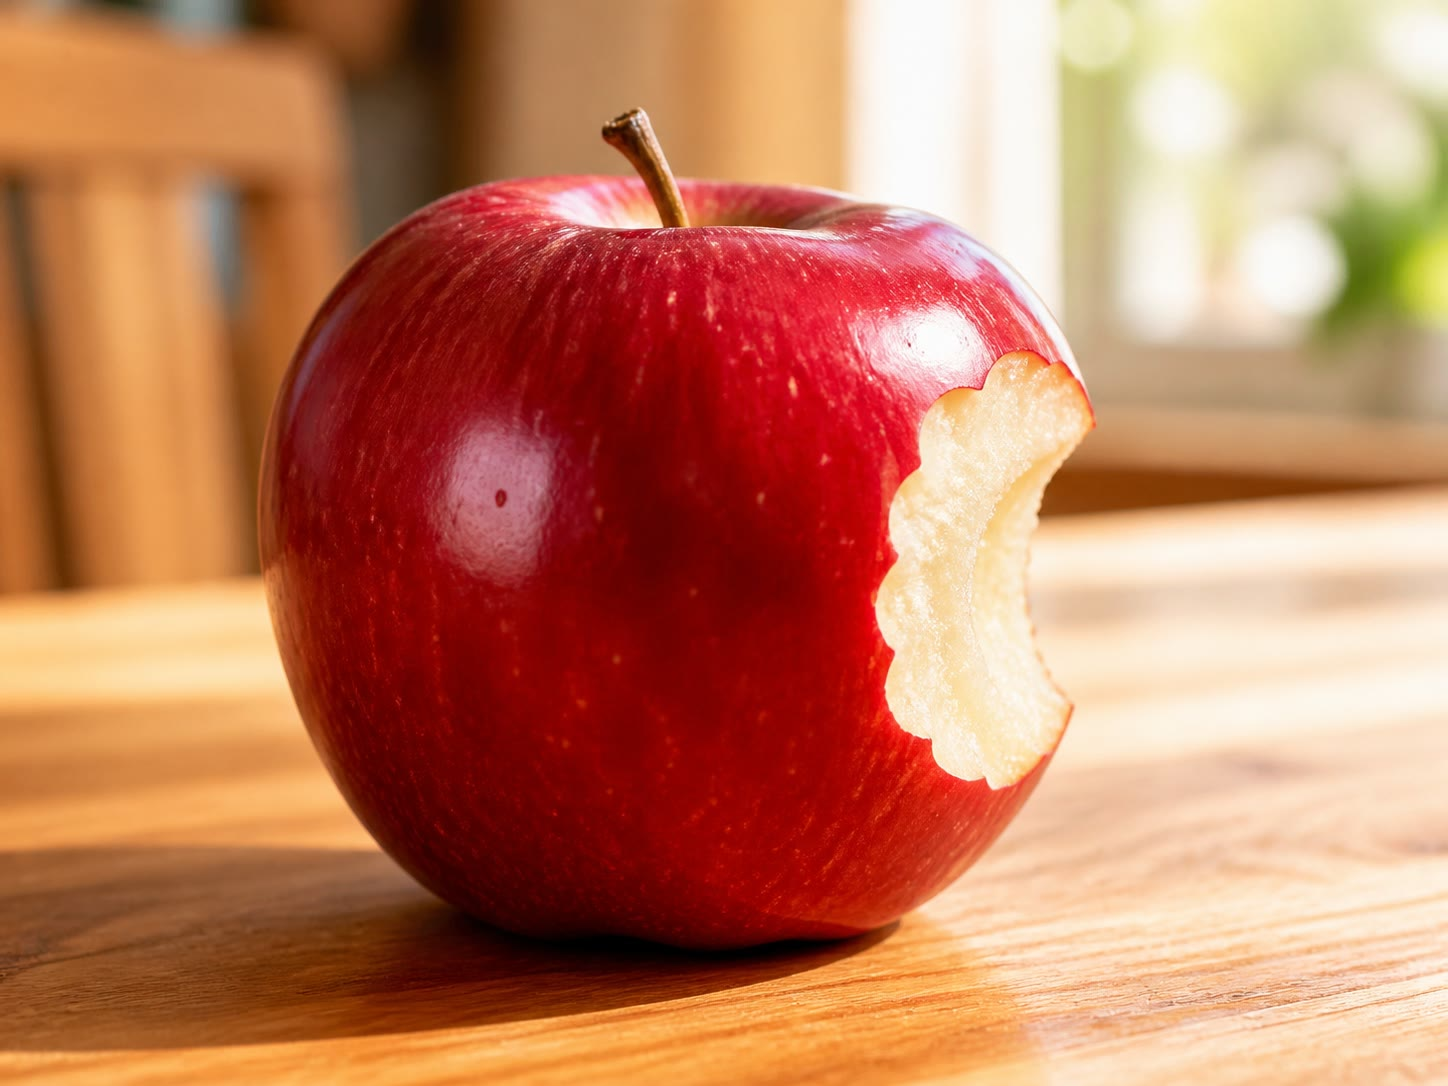
\includegraphics[width=0.52\linewidth]{images/book1/ai/g1-five-senses-apple.jpg}

{\small 一个苹果供五种感官共享：眼睛看见它的红色，手摸到它光滑的表皮，耳朵听见缺掉那一口的咬响，鼻子闻到它的香气，舌头留住了它的味道。}
\end{omfigure}

\begin{example}[试一试：听声散步]\label{ex:g1:five-senses:sounds}
安静地坐着，闭上眼睛，数一数你身边的声音，
数上一小会儿：汽车、说话声、风声和你自己的呼吸。闭上眼睛后，
耳朵会察觉那些忙碌的眼睛让你错过的声音。多数人
会发现 $4$ 或 $5$ 种之前没注意到的声音。
\end{example}

\begin{remark}[感官的保护作用]\label{rem:g1:five-senses:danger}
感官也是守卫。鼻子常常先于眼睛闻到烟味，
而后才看见火；皮肤会让手从热锅上缩回；苦味会提醒：
“不要咽下这个”。绝不要故意去尝或去闻
不认识的东西，先问大人。守卫发挥作用时，
就要小心对待它们。
\end{remark}

\section{仔细观察}

只是看见，还不算观察。每个人都\emph{见过}瓢虫；
谁能说出它有几条腿？

\begin{definition}[观察]\label{def:g1:five-senses:observation}
\emph{观察}\index{观察}是仔细地、有目的地运用感官，
以回答某个问题 --- 然后准确地说出或画出
所注意到的，而不是所预期的。一个
\emph{观察结果}\index{观察结果}是仔细观察
所发现的内容。
\end{definition}

\begin{method}[如何观察]\label{met:g1:five-senses:how}
\begin{enumerate}
  \item 选择一个问题：\emph{瓢虫有几条腿
        ？}
  \item 慢慢地观看（或聆听、触摸），不要着急；
  \item 用准确的词语说出你注意到的内容：不要说“它很小”，
        而要说“它比我的指甲还小”；
  \item 把它画出来或说出来，让别人也能核对。
\end{enumerate}
好的观察结果可以由朋友核对：如果你们两人都看，
你们都应该数出 $6$ 条腿。
\end{method}

\begin{example}[准确的词语]\label{ex:g1:five-senses:words}
比较“这块石头很漂亮”与“这块石头灰色、光滑、
圆润，而且比我的手还凉”。第二句是一个
观察结果：另一个孩子能在整篮石子中
挑出这一块。
\end{example}

\begin{omfigure}
\begin{tikzpicture}[scale=0.8]
  % six legs, three per side
  \draw[thick] (1.32,-0.45) -- ++(-30:0.45);
  \draw[thick] (0.9,-0.76) -- ++(-55:0.45);
  \draw[thick] (0.38,-0.92) -- ++(-75:0.45);
  \draw[thick] (-1.32,-0.45) -- ++(210:0.45);
  \draw[thick] (-0.9,-0.76) -- ++(235:0.45);
  \draw[thick] (-0.38,-0.92) -- ++(255:0.45);
  % body, wing split, spots
  \draw[thick, fill=omDef!12] (0,0) ellipse (1.5 and 0.95);
  \draw[thick, omDef] (0,0.95) -- (0,-0.95);
  \fill[omThm] (-0.55,0.3) circle (0.13);
  \fill[omThm] (-0.85,-0.25) circle (0.13);
  \fill[omThm] (0.5,0.4) circle (0.13);
  \fill[omThm] (0.75,-0.25) circle (0.13);
  % head and antennae
  \fill[omDef] (1.55,0) circle (0.3);
  \draw[thick] (1.75,0.18) .. controls (2.0,0.35) .. (2.1,0.55);
  \draw[thick] (1.78,-0.14) .. controls (2.05,-0.28) .. (2.18,-0.42);
  \node[right, font=\small] at (2.8,0.5)
    {有几个斑点？有几条腿？};
  \node[right, font=\small] at (2.8,-0.5)
    {慢慢看，然后数一数。};
\end{tikzpicture}

{\small 观察瓢虫：仔细的眼睛数出这只虫子有 $4$ 个斑点 ---
而它总是有 $6$ 条腿。}
\end{omfigure}

\section{当感官被欺骗时}

感官非常奇妙，但也会被欺骗。这正是
为什么在后面的章节里，我们要学习如何\emph{测量}。

\begin{example}[两条线段]\label{ex:g1:five-senses:lines}
下图中，哪一条线段更长？几乎每个人都回答
“上面那一条”。现在用一根细绳来检验：这两条线段
其实一样长。眼睛被箭头的
尖端骗了。
\end{example}

\begin{omfigure}
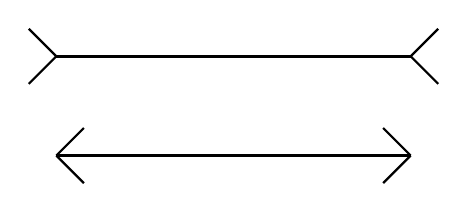
\begin{tikzpicture}[scale=0.9]
  \draw[very thick] (0,1.4) -- (5,1.4);
  \draw[thick] (0,1.4) -- ++(135:0.55) (0,1.4) -- ++(-135:0.55);
  \draw[thick] (5,1.4) -- ++(45:0.55) (5,1.4) -- ++(-45:0.55);
  \draw[very thick] (0,0) -- (5,0);
  \draw[thick] (0,0) -- ++(45:0.55) (0,0) -- ++(-45:0.55);
  \draw[thick] (5,0) -- ++(135:0.55) (5,0) -- ++(-135:0.55);
\end{tikzpicture}

{\small 著名的箭头错觉：两条线段长度相同。
用一根细绳检验一下！}
\end{omfigure}

\begin{example}[动手试一试：三只碗]\label{ex:g1:five-senses:bowls}
请大人准备三碗水：一碗凉的，一碗温的，
一碗温度刚好的暖水。把一只手放在凉水碗里，另一只手放在
暖水碗里，慢慢数到 $20$。然后把两只手
一起放进中间那碗水里：同一碗水，一只手觉得暖，
另一只手却觉得凉！仅靠触觉，无法可靠判断
冷和热 --- 下一章正是要研究这个问题。
\end{example}

\begin{remark}[感官的帮手]\label{rem:g1:five-senses:tools}
人们制造了帮助感官的工具：眼镜和放大镜帮助眼睛，
医生的听诊器帮助耳朵。在本书后面，
被称为\emph{仪器}的工具将帮得更多：
它们会把看和摸变成数数与测量，
而数数要难骗得多。
\end{remark}

\section{练习}

\begin{exercise}[$\star$]\label{exo:g1:five-senses:1}
说出五种感官，并分别指出每种感官
负责这一功能的身体部位。
\end{exercise}

\begin{exercise}[$\star$]\label{exo:g1:five-senses:2}
哪一种感官会告诉你：（a）收音机是否开着？（b）汤
是否太咸？（c）你的套头衫是否扎人？（d）灯
是否灭了？
\end{exercise}

\begin{exercise}[$\star$]\label{exo:g1:five-senses:3}
一块蛋糕正在另一个房间的烤箱里烘烤，烤箱门关着。哪一种感官
最先发现它？等你终于吃到一块时，
你会用到哪些感官？
\end{exercise}

\begin{exercise}[$\star$]\label{exo:g1:five-senses:4}
做\cref{ex:g1:five-senses:sounds}中的声音探索：闭上眼睛，
数一数你周围的声音。你听到了几种？
哪一种声音让你感到意外？
\end{exercise}

\begin{exercise}[$\star$]\label{exo:g1:five-senses:5}
用三个精确的词描述你的鞋子，
如\cref{ex:g1:five-senses:words}所示。“好看”和“漂亮”
都不允许使用！
\end{exercise}

\begin{exercise}[$\star$]\label{exo:g1:five-senses:6}
安娜说：“这只猫很软。”鲍勃说：“这只猫是最好的猫。”
哪一句是观察结果？是哪一种感官得出的？
另一句又是什么？
\end{exercise}

\begin{exercise}[$\star$]\label{exo:g1:five-senses:7}
哪一种感官会警告你以下每种危险：（a）屋里某处有烟；
（b）锅太烫，拿不住；（c）一辆车从你身后驶来？
\end{exercise}

\begin{exercise}[$\star$]\label{exo:g1:five-senses:8}
一位朋友闭上眼睛。你每次把一把勺子、一块海绵和一颗小石子
依次放在他面前。仅凭触觉，他能说出这三样东西吗？
哪一样最容易辨认？
\end{exercise}

\begin{exercise}[$\star\star$]\label{exo:g1:five-senses:9}
看一看\cref{ex:g1:five-senses:lines}中的两条线段。向一位朋友说明
如何在不依靠眼睛的情况下，确定哪一条线段更长。
你的方法还能比较一条线段和一根弯曲的
细绳吗？
\end{exercise}
